\documentclass{standalone}
\usepackage{tikz}
\usepackage{pgfplots}
\pgfplotsset{compat=1.17}

\begin{document}

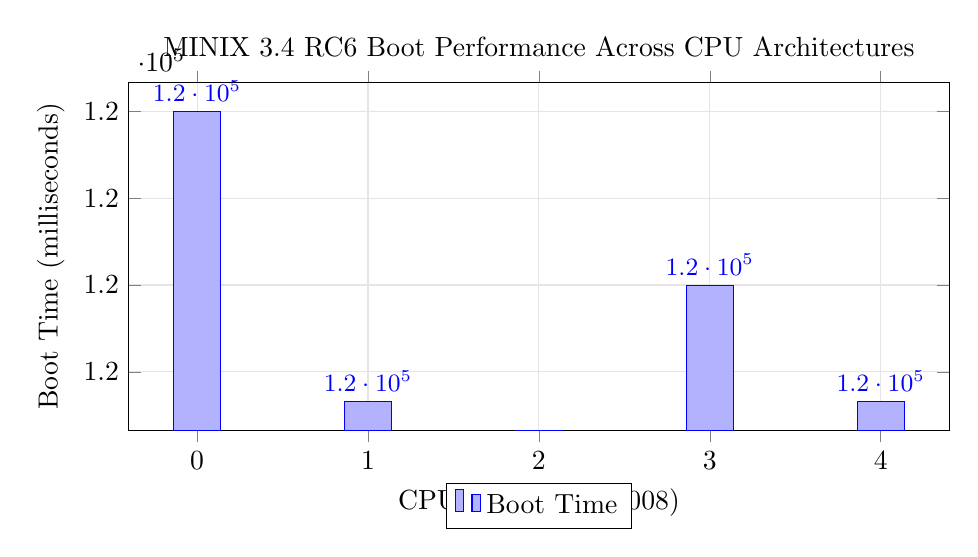
\begin{tikzpicture}
\begin{axis}[
    title={MINIX 3.4 RC6 Boot Performance Across CPU Architectures},
    xlabel={CPU Type (1989-2008)},
    ylabel={Boot Time (milliseconds)},
    ybar,
    bar width=0.6cm,
    width=12cm,
    height=6cm,
    legend style={at={(0.5,-0.15)}, anchor=north, legend columns=-1},
    xtick=data,
    grid=major,
    grid style={gray!20},
    nodes near coords,
    nodes near coords style={font=\small}
]

\addplot coordinates {
    (0, 120008.00)
    (1, 120006.33)
    (2, 120006.00)
    (3, 120007.00)
    (4, 120006.33)
};

\legend{Boot Time}
\end{axis}
\end{tikzpicture}

\end{document}